% !TeX root = ../tfm.tex
%! TEX root = ../tfm.tex
\documentclass[tikz=true]{standalone}
\usepackage[utf8]{inputenc}

\usepackage{tikz}
\usepackage{amsfonts}
\usepackage{amsmath,amssymb}
\usepackage{systeme,mathtools}
\usetikzlibrary{positioning,arrows,quotes}
\usetikzlibrary{shapes, decorations}
\usetikzlibrary{bayesnet}
\tikzset{>=latex}

\begin{document}
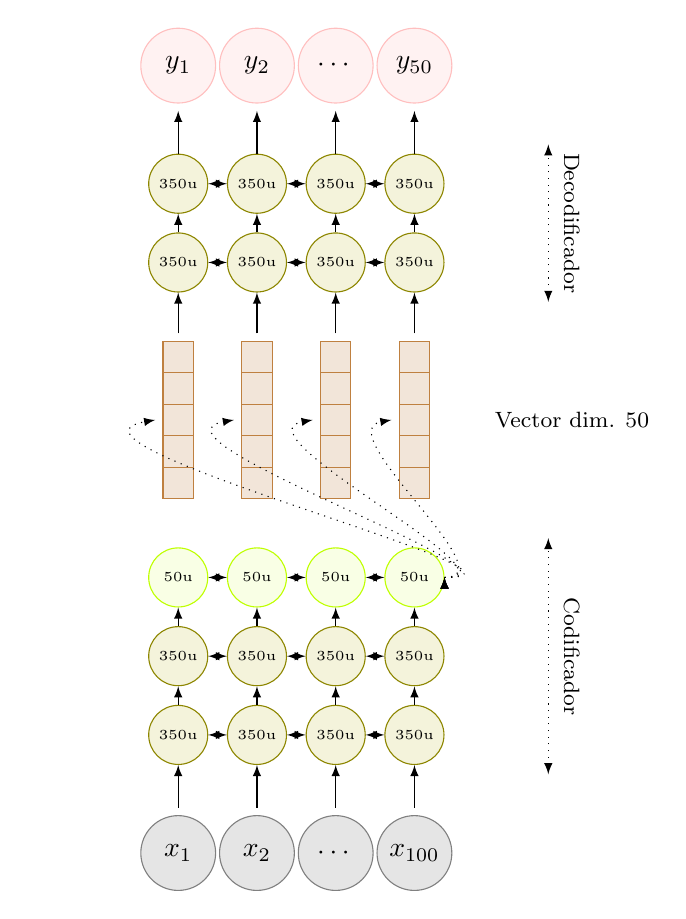
\begin{tikzpicture}[node distance = 1.5mm, auto,
gru/.style={
  circle,draw=#1,fill=#1!10,inner sep=0pt, minimum size=0.75cm
},
inout/.style={
  circle,draw=#1,fill=#1!20,inner sep=0pt,minimum size=0.95cm, outer sep=1mm
},
vec/.style={
  rectangle split, draw=#1, rectangle split parts=5,fill=#1!20, outer sep=1mm 
}]


% Entradas

\foreach \input [count=\inpos from 1] in { {$x_1$}, {$x_2$}, {$\cdots$}, {$x_{100}$} }{
  \node[inout=gray] (in\inpos) at (\inpos, -0.5) {\input};
}

\foreach \encoderstep in {1,2,3,4}{
  %ENCODER
  % 2* Bidir
  \foreach \encoderlevel in {1,2,7,8}{
    \node[gru=olive] (enc\encoderlevel\encoderstep) at (\encoderstep, \encoderlevel) {\tiny 350u};
  }
  % Salida encoder
  \node[gru=lime] (enc3\encoderstep) at (\encoderstep, 3) {\tiny 50u};
  
  \draw[arrows=->] (in\encoderstep) -- (enc1\encoderstep);
  \draw[arrows=->] (enc1\encoderstep) -- (enc2\encoderstep);
  \draw[arrows=->] (enc2\encoderstep) -- (enc3\encoderstep);
  \draw[arrows=->] (enc7\encoderstep) -- (enc8\encoderstep);

  \node[vec=brown] (vector\encoderstep) at (\encoderstep, 5) {};
  \draw[arrows=->] (vector\encoderstep) -- (enc7\encoderstep);
}

% Bidirs
\foreach \hiddenlevel in {1,2,3,7,8}{
  \draw[arrows=<->] (enc\hiddenlevel1) -- (enc\hiddenlevel2);
  \draw[arrows=<->] (enc\hiddenlevel2) -- (enc\hiddenlevel3);
  \draw[arrows=<->] (enc\hiddenlevel3) -- (enc\hiddenlevel4);
}

%Salidas
\foreach \output [count=\outpos from 1] in { {$y_1$}, {$y_2$}, {$\cdots$}, {$y_{50}$}} {
  \node[inout=pink] (in\outpos) at (\outpos, 9.5) {\output};
  \draw[arrows=->] (enc8\outpos) -- (in\outpos);
}

\foreach \encvec in {1,2,3,4} {
  \draw[thin,dotted,arrows=->] (enc34.east) edge[=>,out=0,in=190] (vector\encvec.west);
}

\node[rotate=-90] at (6,2) {\footnotesize Codificador};
\draw[dotted,arrows=<->] (5.7,0.5) -- (5.7,3.5);
\node[rotate=-90] at (6,7.5) {\footnotesize Decodificador};
\draw[dotted,arrows=<->] (5.7,6.5) -- (5.7,8.5);
\node at (6,5) {\footnotesize Vector dim. 50};

\end{tikzpicture}
\end{document}
